%% 
%% Copyright 2007-2020 Elsevier Ltd
%% 
%% This file is part of the 'Elsarticle Bundle'.
%% ---------------------------------------------

\documentclass[preprint,12pt,authoryear]{elsarticle}
%\usepackage{natbib}
%% Use the option review to obtain double line spacing
%% \documentclass[authoryear,preprint,review,12pt]{elsarticle}

%% Use the options 1p,twocolumn; 3p; 3p,twocolumn; 5p; or 5p,twocolumn
%% for a journal layout:
%% \documentclass[final,1p,times,authoryear]{elsarticle}
%% \documentclass[final,1p,times,twocolumn,authoryear]{elsarticle}
%% \documentclass[final,3p,times,authoryear]{elsarticle}
%% \documentclass[final,3p,times,twocolumn,authoryear]{elsarticle}
%% \documentclass[final,5p,times,authoryear]{elsarticle}
%% \documentclass[final,5p,times,twocolumn,authoryear]{elsarticle}

%% For including figures, graphicx.sty has been loaded in
%% elsarticle.cls. If you prefer to use the old commands
%% please give \usepackage{epsfig}

%% The amssymb package provides various useful mathematical symbols
\usepackage{amssymb}
%% The amsthm package provides extended theorem environments
\usepackage{amsthm}

%% The lineno packages adds line numbers. Start line numbering with
%% \begin{linenumbers}, end it with \end{linenumbers}. Or switch it on
%% for the whole article with \linenumbers.
%% \usepackage{lineno}

\journal{Atmospheric Environment}


\begin{document}

\begin{frontmatter}

%% Title, authors and addresses

%% use the tnoteref command within \title for footnotes;
%% use the tnotetext command for theassociated footnote;
%% use the fnref command within \author or \affiliation for footnotes;
%% use the fntext command for theassociated footnote;
%% use the corref command within \author for corresponding author footnotes;
%% use the cortext command for theassociated footnote;
%% use the ead command for the email address,
%% and the form \ead[url] for the home page:
%% \title{Title\tnoteref{label1}}
%% \tnotetext[label1]{}
%% \author{Name\corref{cor1}\fnref{label2}}
%% \ead{email address}
%% \ead[url]{home page}
%% \fntext[label2]{}
%% \cortext[cor1]{}
%% \affiliation{organization={},
%%            addressline={}, 
%%            city={},
%%            postcode={}, 
%%            state={},
%%            country={}}
%% \fntext[label3]{}

\title{Chemical composition and mass closure for PM2.5 in Buenos Aires}

%% use optional labels to link authors explicitly to addresses:
%% \author[label1,label2]{}
%% \affiliation[label1]{organization={},
%%             addressline={},
%%             city={},
%%             postcode={},
%%             state={},
%%             country={}}
%%
%% \affiliation[label2]{organization={},
%%             addressline={},
%%             city={},
%%             postcode={},
%%             state={},
%%             country={}}

\author{Pablo Lichtig, Facundo Baraldo, Julián Gelman Constantín, Diego Alessandrelo, Marcelo de Otto, Melisa Diaz Resquín, Facundo Bajano, Ramiro Espada, Cristina Rössler,  Daniela Santágata, Héctor Bajano,  Darío Gómez, Laura Dawidowski}

%\affiliation{organization={},%Department and Organization
%            addressline={}, 
%            city={},
%            postcode={}, 
%            state={},
%            country={}}

\begin{abstract}
%% Text of abstract

Mass reconstruction tries to achieve closure between gravimetric mass and the sum of major components to account for unmeasured species. PM mass reconstruction is used to identify and correct potential measurement errors and estimate source contributions (\cite{Chow2015MassReview}). The practice of mass closure is key in checking internal consistency and validating chemical analysis results. It's use for chemical characterization studies is highly recommended%, particularly if additional techniques (i.e. receptor models) are to be used for determining source contributions to particulate matter%
. One particular species is ammonium:  it is an important constituent of particulate mass in the atmosphere, but it is well known to be difficult to quantify due to possible sampling artifacts. Losses of semivolatile species such as $\mathrm{NH_4 NO_3}$ can be particularly problematic. In order to evaluate ammonium losses from aerosol particles collected on filters, a series of experiments were conducted to obtain more precise mass closure results.

Two 24-hour samples were collected every 3 days for almost a year, one in a quartz fiber high volume (HV) filter and another one in a Teflon (Polytetrafluoroethylene) low volume (LV) membrane filter in a measuring site in Buenos Aires. Each filter was dried and weighted, and HV filters were cut to perform different chemical analyses, including Elemental Carbon/Organic Carbon, ions and trace elements.

%Resultados y conclusiones


\end{abstract}

%%Graphical abstract
\begin{graphicalabstract}
%\includegraphics{grabs}
\end{graphicalabstract}

%%Research highlights
\begin{highlights}
\item Research highlight 1
\item Research highlight 2
\end{highlights}

\begin{keyword}
%% keywords here, in the form: keyword \sep keyword
Particulate Matter \sep PM2.5 \sep air pollution \sep air quality \sep EC/OC \sep filter
%% PACS codes here, in the form: \PACS code \sep code

%% MSC codes here, in the form: \MSC code \sep code
%% or \MSC[2008] code \sep code (2000 is the default)

\end{keyword}

\end{frontmatter}

%% \linenumbers

%% main text
\section{Introduction}
\label{sec:introduction}

Air pollution represents one of the greatest environmental risks to health. According to the World Health Organization, in 2012 one out of every nine deaths was the result of air pollution-related conditions, and 3 million of those are attributable to outdoor conditions. Aerosols, and particularly particulate matter of a diameter less than 2.5 micrometers (PM$_{2.5}$) is especially relevant when assessing human exposure to pollution (\cite{WorldHealthOrganization2016AmbientDisease}). In Argentina, WHO estimates about 14,800 deaths in 2016 (\cite{WorldHealthOrganization2018AmbientDeaths}).

Knowing aerosol composition is useful to apportion sources, evaluate pollution causes, assess toxic components which may be of interest for public health, evaluate particle scattering and absorption and its effects on visibility and the Earth's radiation balance. %Agregar short lived climate forcers y climate change, (Caerbonosas, SO2, NH4+).
This proceeding usually consist in quantifying many aerosol components, and attempting to reconstruct aerosol mass by using specific equations (a proceeding often known as mass closure). However, when using filters, measurements are not artifact free. Of particular importance are the facts that ammonium an nitrate (which are present in all mass closure equations) may evaporate from Teflon and quartz filters. Another usual problem is the conversion from organic carbon (OC) to organic matter (OM).%, which requires a multiplier ($f$) that may range from 1.2 to 2.6, depending on OM oxidation, although usually 1.4 is used for urban sites.  \cite{Chow2015MassReview}  --> Va a métodos

MABA is the third largest city in the LAC region (after S\~ao Paulo and Mexico City). It is a flat terrain, located on the southwestern shore of the La Plata River at $\sim$200 km from the South Atlantic Ocean. It has relatively high wind speeds all year round, so that the atmosphere is cleaned and renewed daily, as traffic slows down during the night \cite{Bogo1999ContinuousCity}. Previous campaigns (\cite{Resquin2018LocalAires}), %HAY CITA PARA LA DE VICKY?)
have measured Equivalent Black Carbon (EBC) and ???????????. However, Elemental/Organic Carbon (EC/OC) and ???? ???? ???? ions have never been measured. %Previous measurements also lack any account for ammonium and nitrate volatility. 

Having good quality, reliable data is also of the utmost importance when evaluating pollution models and regional variability. %CITA
A usual problem is that different measuring techniques and filter materials can shed different results. However, regional pollution assessments require knowledge of multiple measuring points. It is therefore important to employ standardized measuring techniques (both in sample collection and sample characterization). The Regional  Cooperative  Arrangements  for  the  Promotion  of  Nuclear Science and Technology in Latin America (ARCAL) is a Cooperation Agreement signed in the scope of the International Atomic Energy Agency. The ARCAL RLA-7023%Revisar número
%Tabla, la hace Laura
project consists in a year-long aerosol measuring campaign in as many as 12 megacities in the Latin America and Caribbean (LAC) region, with as close as possible methodologies, taking into account local capabilities and enhancing them if possible. 

This study consists on an analysis of the results of this campaign in the Metropolitan Area of Buenos Aires (MABA). With almost a year of measurements and characterization of filters (from April 3rd 2019 to March 16 2020, when mandatory quarantine in Argentina stopped the measurements), it is the most complete research on PM$_{2.5}$ in recent times. It is also, as far as we could find, the first study to take into explicit account NH$_4^+$ volatility, and to measure EC/OC and ?????????? ?????? ions.
It is important to highlight that the purpose of the paper is to show a preliminary study of NH$_4^+$ evaporation loss and it is a starting point to continue working more in detail about the subject in the future because the results here shown are very encouraging but more variables have to take into account for a proper study.


%- Buenos Aires, que es llano, que en términos generales hay renovación diaria (paper de Bogo). Describir las campañas previas en Buenos Aires (Marina, Vicky, Melisa) qué se dijo y qué no se dijo previamente (No hay determinaciones de OC ni tampoco de EC con termoptico - creo que algunos iones que nos midieron en Costa Rica nunca los habíamos medido acá - Las mediciones previas no contemplaban la volatilidad del amonio… este párrafo hay que trabajarlo, porque la mayor parte de los datos son nuestros) --> MEJORAR Y MUCHO

%- Revisión historia de las ciudades ARCAL (Atmospheric Environment Volume 189, September 2018, Pages 187-212) --> El paper es de china, ¿no? ¿La idea sería copiar la forma en que describe? Tiene sentido siendo que hicimos sólo Bs As?
%- Un párrafo indicando la necesidad de contar con una mirada regional con técnicas estandarizadas. Breve descripción del proyecto ARCAL: ciudades, objetivos, metodología cómun, la existencia de un protocolo de muestreo. 

%Describir lo que hicimos sin detalles y porqué lo hicimos (o sea, en qué se aporta a las dificultades antes indicadas)
%Siguiendo lo que se dijo en (1) , pero ahora sí indicando la estrategia en Buenos Aires para medir los compuestos químicos con nuestros equipos, describir que la campaña
%en Buenos Aires se realizó entre xx (Período de muestreo) y se determinaron xx, xxx, xxx y xxx por tal y tal y cual técnica. Decir que se mide por primera vez OC y EC, y que
%se mide (creo que algún ion también por primera vez, que lo midieron en Costa Rica)
%También se midió Mercurio, fíjate Facu, comparalo con nuestros trabajos (Darío + Patricia+ Marina + Victoria).
%Después contar que con el objetivo de mejorar la reconstrucción másica se identificó la dependencia en el tiempo de la volatilidad del amonio. Una vez que tengamos los resultados, mejoramos este párrafo, por ahora lo dejamos medio así.



\section{Methods}
\label{sec:methodology}
\subsection{Sample collection}
As part of the ARCAL project, the monitoring strategy consisted in sample collection with both quartz high volume (HV) filters and Teflon low volume filters (LV). In Buenos Aires, a single sampling site was selected.

%\subsubsection{Sampling site} %Es casi una copia del que mandó Darío, hay que editarlo para que no salte cosas de plagio.
All samples were collected on the roof of a building at Comisión Nacional de Energía Atómica (CNEA, 34.57°S, 58.51°W), similar to \cite{GelmanConstantin2021Plasma-basedAerosols}, which is approximately 12 m above sea level, in the Greater Buenos Aires. The roof selected to place the sampler is at approximately 25 m distance from the highway that divides the city of Buenos Aires from surrounding districts. It is normally influenced by emissions from urban vehicular traffic, sea salt spray, local and regional biomass burning \cite{Resquin2018LocalAires}.



%\subsubsection{Sampling strategy}
%Falta colocar los equipos que usamos, tenemos el problema de que para LV fuimos cambiando de equipo a medida que pasaba el tiempo.
Samples were collected during a 24 hour period, starting at noon for safety and operational reasons. A sample was collected every 3 days. All were labeled according to the day sampling started.
LV filters were 47 mm, with a 4 $\mu$m pore, %CHEQUEAR ESTO, ES LO QUE DICE EL PROTOCOLO PERO CREO QUE ESTÁ MAL
and a collection efficiency of at least 99.9\%. Due to multiple equipment breakage, some filters were measured with a Partisol \textbf{COMPLETAR}, and some with a PQ \textbf{COMPLETAR}, some with an Airmetric \textbf{COMPLETAR}. Taking that into account, we used HV filters for most of the analysis (due to LV filters being present in most regulations, some measurements and comparisons are still shown). 

HV filters were (20.3 $\pm$ 0.2) cm x (25.4 $\pm$ 0.2) cm in size, with and exposed area of 406.5 cm$^2$, and a collection efficiency of at least 99\% according to the ASTM D 2986-91 test.



Every filter was dried for 24 hours, with a relative humidity lower than 50\% and a temperature lower than 30 °C. HV filter mass was measured in a Sartorius %chequear modelo
analytical weighing scaled, able to measure up to 0.01 mg. LV filters were weighted using a METTLER TOLEDO %chequear modelo, aclarar con qué se desestatiza
ultramicrobalance, with a readability of up to 0.1 $\mu$g. The same weighting procedure was employed before and after sampling. Blank HV filters were heated at least 6 hs at 600 °C %mufla=furnace
to get rid of spurious organic matter, just before stabilization in a dryer and weighting. 
HV samples were transported in an hermetically sealed bag, after being bent so that the side with the sample was not exposed. The bags were further protected from light with aluminum foil. LV filters were transported in a sealed petri dish, to prevent contamination.

After being weighted, HV used filters were cut with a cutter designed \emph{ad hoc} according to EPA norms. %A larger piece was sent refrigerated from Buenos Aires to San Jos\'e de Costa Rica for EC/OC and ions measurement, while further pieces were kept in Buenos Aires so as to further measure ions and metals.    EC/OC, iones, PAH, etc. "Se cortó en 9 piezas para múltiples análisis químicos".

When not in the dryer, HV filters were kept at -20 °C, and LV at normal refrigerator temperature ($\sim$ 4--8 °C). $\mathrm{NH_4^+}$ was measured as quickly as possible, to minimize mass loss.


\subsection{Filter composition}
%FACU o Costa Rica (habría que ver como preparan para OC/EC)
For ion analysis, cut filters are placed in a 150 ml beaker and extracted with
deionized water, using an ultrasonic bath at 45 °C for 45 minutes, with 15 minute intervals for renewal of the ultrasound bath in between. The extract obtained is quantitatively transferred to a 100 ml flask. The analysis of the ions was carried out through suppressed ion chromatography with the equipment DIONEX ICS-5000, a ION PACK AS19 - Analytical - 4 x 250 mm column and KOH as eluent.
In the case of the trace elements, a digestion procedure for microwave extraction was performed. 10 ml of a acid solution of  3\% $\mathrm{HNO_3}$/8\% $\mathrm{HCl}$ are added to the centrifuge tubes with the cut filters inside. After the microwave extraction, the sample is dispensed in a 20 ml beaker and analysed with an inductively coupled plasma mass spectrometry equipment (ICP-MS) Perkin Elmer Optima 5100 DV.
%Referencia de la norma 
%Lo de Costa Rica?

\subsection{Mass reconstruction}
Mass reconstruction was attempted according to \textbf{ELEGIR} method. [Si] was estimated as $2.4729$\ [Al] (\textbf{CITA}). 
\subsection{Ammonium conservation study}

A preliminary experimental system was designed to measure the evaporation loss of ammonium during the storage of the cut filter since it is conserved up to when it´s measured. The idea was to be able to quantify the correctly the the NH$_4^+$ when for any circumstance the ion analysis couldn't take place right after the cutting of the filter. 

A HV filter was cut but instead of it´s pieces being measured by different techniques, all of them where stored in the freezer and analysed by ion chromatography in different days, during the lapse of 263 hours. It´s important to notice that this experiment took place only in June 2019 and that the filter was sampled the day XXX, meaning that more test have to take place for a meaningful result to take in count more variables such as the concentration of ammonium in the atmosphere the sampling day.

It is also worth noticing that this study cannot revert artifacts due to losses that happened during sampling or drying. These, however, do not affect mass closure, since they are already present when the filter is weighted.

\section{Results and discussion}
\label{sec:results}

\subsection{PM$_{2.5}$ mass}

\label{subsec:total_mass}
In Figure \ref{fig:PM2.5_mass} we show the temporal series of HV and LV filters. As expected [\textbf{CITA}], in all cases HV PM$_{2.5}$ measurements were higher than LV PM$_{2.5}$. As expected, the mass concentration follows a lognormal distribution (see \ref{subsec:resreconstruction} for a description of the tests).

HV mass concentrations and LV mass concentrations are linearly related \ref{fig:hv_lv}.
%ver si esto va acá o en metodología

 \begin{figure}[h!]
     \centering
     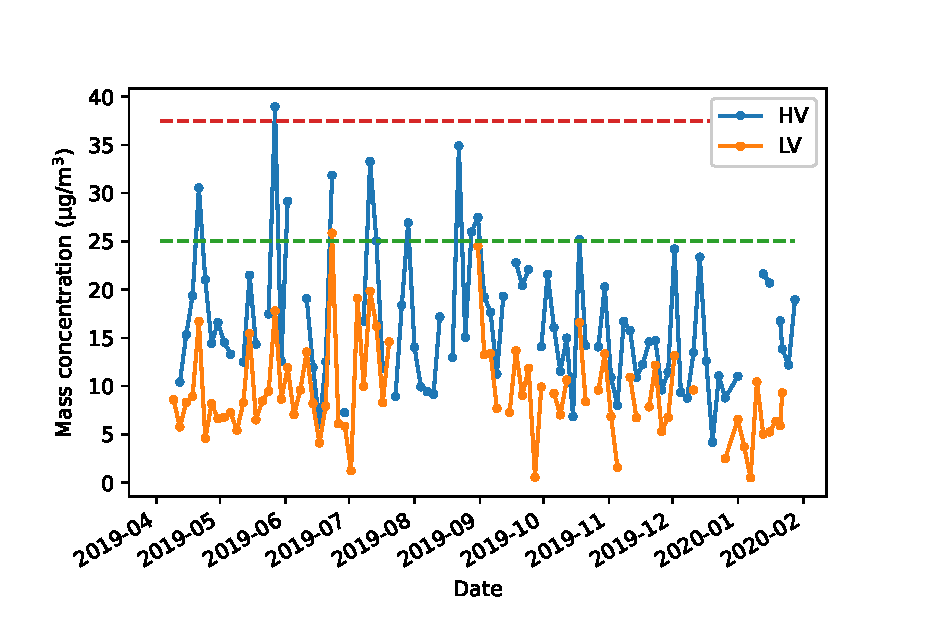
\includegraphics[width=0.7\textwidth]{time_series.eps}
     \caption{High volume and Low Volume measurements during the campaign. As shown, HV filters usually register higher PM$_{2.5}$ mass concentration than LV. Dashes in red show target 3, and dashes in green show best known upper limit, according to WHO Guidelines \textbf{CITA}.} 
     \label{fig:PM2.5_mass}
 \end{figure}
 
 \begin{figure}[h!]
     \centering
     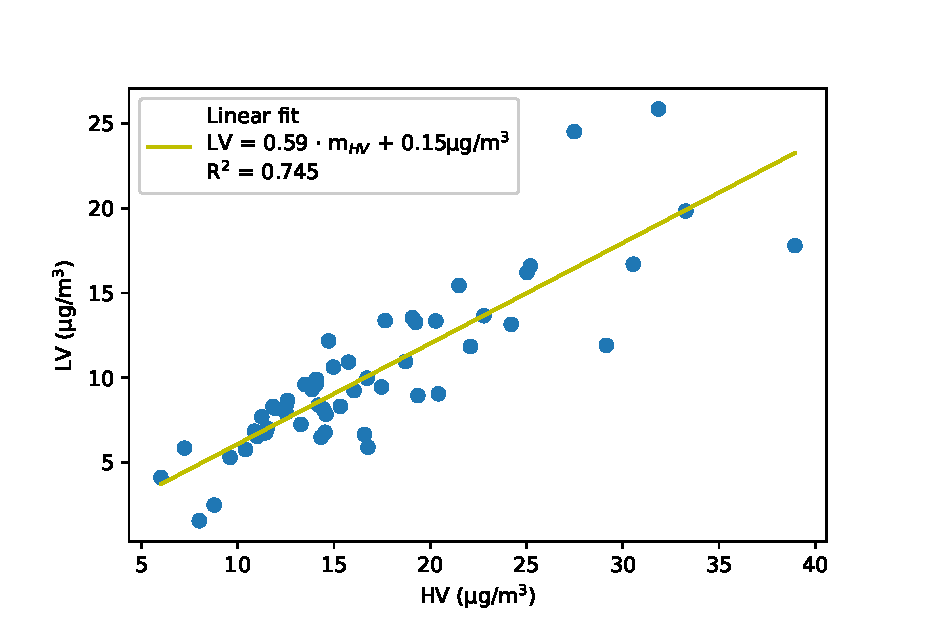
\includegraphics[width=0.5\textwidth]{lv_vs_hv.eps}
     \caption{LV vs HV PM$_{2.5}$. There is a linear relationship between the to variables (R$^2 = 0.745$, with larger dispersion at higher PM$_{2.5}$ mass. }
     \label{fig:hv_lv}
 \end{figure}
 
 During the measured year, HV filters showed values surpassing guidelines 10 times, and LV filters did so twice.  The yearly mean value was $10.2 \:  \mathrm{\mu g\, m^{-3}}$, SD = $4.8$ for LV and $16.9\: \mathrm{\mu g\, m^{-3}}$, SD = $7.0\: \mathrm{\mu g\, m^{-3}}$. Maximum 24-hour values were $38.2 \: \mathrm{\mu g\, m^{-3}}$ for HV filters and $25.9\: \mathrm{\mu g\, m^{-3}}$ for LV. Taking into account that WHO guidelines recommend less than $25\; \mathrm{\mu g\, m^{-3}}$ for 24-hour mean values, and less than $10\: \mathrm{\mu g\, m^{-3}}$ for annual means, there is a noticeable difference in compliance if HV or LV filters are taken as the standard (although LV values should be considered with some precaution in this particular study). 
 
Seasonal averages (shown for HV filters in table \ref{tab:seasonal_pm}) show maximum PM values in autumn and winter, with lower values in spring and summer. 

\begin{table}[h]
    \centering
    \begin{tabular}{c c c}
        \hline
        Season & Mean $\left(\mathrm{\mu g\, m^{-3}}\right)$ & StDev $\left(\mathrm{\mu g\, m^{-3}}\right)$\\\hline \hline
        DJF & 16.7 & 6.3\\
        MMA & 18.5 & 6.7\\
        JJA & 18.1 & 8.7\\
        SON & 15.4 & 4.7\\ \hline
    \end{tabular}
    \caption{Seasonal PM2.5 average of HV filter during sampling year.}
    \label{tab:seasonal_pm}
\end{table} % Ver si esto tiene sentido. MMA en realidad corta años, lo que siendo que es un año solo es raro conceptualmente. Pensar qué hacer con eso
 
 %WHO Guidelines do not stipulate which measurement method should be used. Even though both EPA and 
% \subsection{Low Volume vs. High Volume}
% According to our measurements, HV filter sampling generally registers higher PM$_{2.5}$ concentrations than LV (fig. \ref{fig:PM2.5_mass}). The relation between LV and high-volume seems linear, even though the R$^2$ parameter is somewhat low (figure \ref{fig:hv_lv}). 
% 
% 
% \begin{figure}
%     \centering
%     \includegraphics[width=\textwidth]{hv_vs_lv_py.png}
%     \caption{HV vs LV PM$_{2.5}$. When looking at the }
%     \label{fig:hv_lv}
% \end{figure}
% 
% \begin{table}[]
%     \centering
%     \begin{tabular}{c|c}
%          &  \\
%          & 
%     \end{tabular}
%     \caption{Caption}
%     \label{tab:my_label}
% \end{table}
\subsection{Mass reconstruction}
\label{subsec:resreconstruction}
PM$_{2.5}$ and all its measured components, with the exception of Fe, Zn and Ag, follow a lognormal distribution according to Python's scypy.stats function ``normaltest'', based on D'Agostino's and Pearson's method (\textbf{CITA}) (the lognormality null hypothesis was rejected if p-$value < 0.05$). %sospecho que esta descripción va en metodología

\subsection{Uncertainty estimation}
\label{subsec:resuncert}

The uncertainty study is based on the evaluation of the parameters that could affect the analytical determination. Taking into account the main uncertainty sources for the analysis, an approximation could be assessed theoretically. This calculation procedure is called uncertainty propagation and was used for the determination of the uncertainty associated with the concentration of the chemical components of the PM.

\subsection{Ammonium conservation study}


 \begin{figure}[h!]
     \centering
     \includegraphics[width=0.8\textwidth]{doc/Amonio.png}
     \caption{Stability of the ammonium during 266 hours of conservation }
     \label{fig:amonio}
 \end{figure}

%\section{Discussion}
%\label{sec:discussion}


\section{Conclusion}
\label{sec:conclusion}
%% The Appendices part is started with the command \appendix;
%% appendix sections are then done as normal sections
%% \appendix

%% \section{}
%% \label{}

%% If you have bibdatabase file and want bibtex to generate the
%% bibitems, please use
%%
\bibliographystyle{elsarticle-harv} 
%%  \bibliography{<your bibdatabase>}

%% else use the following coding to input the bibitems directly in the
%% TeX file.



%% \bibitem[Author(year)]{label}
%% Text of bibliographic item
\bibliography{references.bib}


\end{document}

\endinput
%%

%The mass concentration of secondary organic aerosols (SOA) was estimated by SOA = (OC – EC × (OC/EC) min ) ∗1.6 using the traditional OC/EC minimum ratio method ( Strader et al., 1999 ; Wu et al., 2009 ), and the mass concentration of primary organic aerosols (POA) was there- after calculated by POA = OC ∗1.6 – SOA . \cite{Ahmad2021ChemicalPakistan}

%Reconstruccion (NH4)2SO4 y esas cosas, y reconstrucción másica sin SiO2, \cite{Cheng2021SourceChina}

% Fujiwara da donde se genera más de cada metal
 %ve otras ecuaciones de reconstruccion masica

%% End of file `elsarticle-template-harv.tex'.
